\documentclass[10pt]{article}
% RATISS Labs — shared preamble (Tectonic / LaTeX)
\usepackage[a4paper,margin=2.3cm]{geometry}
\usepackage{xcolor}
\usepackage{graphicx}
\usepackage{booktabs}
\usepackage{amsmath}
\usepackage{microtype}
\usepackage[hidelinks]{hyperref}
\definecolor{ratiss}{RGB}{14,107,102}
\definecolor{ratisslight}{RGB}{238,252,249}
\definecolor{inkgray}{RGB}{74,111,107}
\hypersetup{colorlinks=true,linkcolor=ratiss,urlcolor=ratiss,citecolor=ratiss}
\setlength{\parindent}{0pt}
\setlength{\parskip}{5pt}
\renewcommand{\familydefault}{\sfdefault}
\newcommand{\ratisshead}[4]{%
  {\color{ratiss}\rule{\linewidth}{1.2pt}}\vspace{6pt}\\
  {\LARGE\bfseries #1}\\[4pt]
  {\large #2}\\[2pt]
  {\color{inkgray}\small #3}\\[2pt]
  {\color{inkgray}\small #4}\vspace{8pt}\\
  {\color{ratiss}\rule{\linewidth}{0.6pt}}\vspace{10pt}%
}
\newcommand{\kwsection}[1]{\section*{\color{ratiss}#1}\addcontentsline{toc}{section}{#1}}
\newcommand{\sourcefoot}{%
  \vspace{10pt}{\color{ratiss}\rule{\linewidth}{0.6pt}}\vspace{4pt}\\
  {\color{inkgray}\scriptsize RATISS Labs --- independent, single-author laboratory, Yaoundé (Cameroon).
  No number in this document is invented: every value carries a source in
  Section~``Data and code availability'' or in the references.
  Negative results are published with the same prominence as positive ones.}%
}

\begin{document}
\ratisshead
{RATISS-ETALONS: Four Computational Standards with Criteria Sealed Before Execution}
{Jonathan Evina --- RATISS Labs, Yaoundé, Cameroon}
{Research object \texttt{ratiss-etalons-004} · version v1 · 2026-09-26 · status: published}
{Repository: \url{https://github.com/jonathansearch/RATISS-ETALONS} (seal 23/23, MIT)}

\kwsection{Abstract}
Four standards --- percolation, 2D Ising, three-body problem, close packings --- were
defined with criteria frozen \emph{before} execution (\texttt{PROTOCOLE.md}).
The score moved from 11/16 to 14/16 after declared corrections. Two reds are kept on
purpose and diagnosed: E01-P2, whose hypothesis ``hole-density peak at $p_c$'' is
INVALID ($h(p)$ is monotone), and E04-P4, where the 3D compressor underestimates
($0.61403$ vs $0.64 \pm 0.020$) because of finite size and a partially crystalline
state ($\psi_6 = 0.827 / 0.935$). Key values: $p_c = 0.0006$; $d_f = 1.8934 \pm 0.0192$;
$T_c = 2.2613$; $\gamma/\nu = 1.7540$; $\Delta E/E = 1.21\times10^{-15}$;
FCC $= 4.44\times10^{-16}$; Burrau $\lambda = 0.55402$ stable at 0.78\%.

\kwsection{Scientific question}
Can a battery of standards with pre-sealed criteria serve as a reproducible reference
to judge every future RATISS computation engine?

\kwsection{Method}
Criteria frozen in \texttt{PROTOCOLE.md} before any run; executions afterwards; every
gap published, including failures. Figures use matplotlib without emoji (lab law).

\begin{figure}[h]\centering
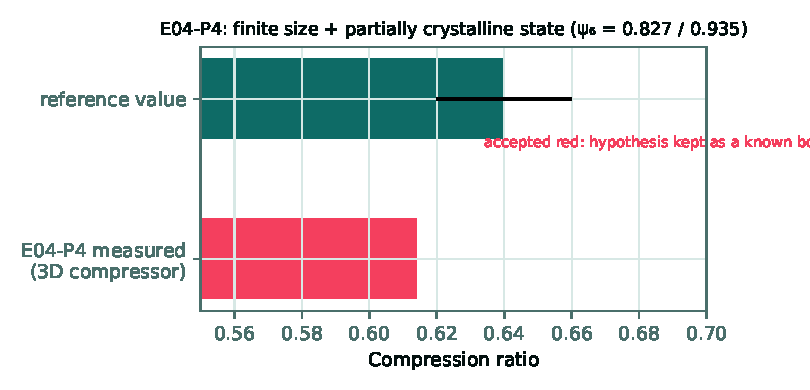
\includegraphics[width=0.85\linewidth]{fig/etalons-e04.pdf}
\caption{E04-P4: measured 3D compression ratio against the reference value with its
uncertainty. The red is accepted as a known bound of the engine.}\label{fig:e04}
\end{figure}

\kwsection{Results}
\begin{itemize}
  \item Score 11/16 $\rightarrow$ 14/16 after declared corrections; seal 23/23.
  \item $p_c = 0.0006$; $d_f = 1.8934 \pm 0.0192$; $T_c = 2.2613$; $\gamma/\nu = 1.7540$.
  \item Conservation: $\Delta E/E = 1.21\times10^{-15}$; FCC lattice $4.44\times10^{-16}$.
  \item Burrau $\lambda = 0.55402$, stable at 0.78\%.
\end{itemize}

\kwsection{Negative results (kept on purpose)}
\begin{itemize}
  \item E01-P2: hypothesis ``hole-density peak at $p_c$'' INVALID --- $h(p)$ monotone.
  \item E04-P4: compressor underestimated, $0.61403$ vs $0.64 \pm 0.020$
        ($\psi_6 = 0.827 / 0.935$, partially crystalline) --- Figure~\ref{fig:e04}.
  \item Fixed-step RK4 FALSIFIED as a standard: $\lambda = +44\,124$, i.e.\ noise.
\end{itemize}

\kwsection{Controls}
Criteria sealed before runs; seal fingerprints 23/23; corrections declared, never silent.

\kwsection{Reproducibility}
\texttt{PROTOCOLE.md} plus repository scripts (commits c230b65, 776658a, b86d027, 8c12b73).

\kwsection{Limitations}
Finite sizes; the two reds are conserved voluntarily as known bounds of the engine.

\kwsection{Data and code availability}
\url{https://github.com/jonathansearch/RATISS-ETALONS};
narrative source: RATISS-ARCHIVES, update of 27/09 section A. Zenodo DOI: to be assigned.

\sourcefoot
\end{document}
